\documentclass[a4paper,11.5pt]{article} % тип документа


%%%Библиотеки
	%\usepackage[warn]{mathtext}	
	\usepackage[T2A]{fontenc} % кодировка
	\usepackage[utf8]{inputenc} % кодировка исходного текста
	\usepackage[english,russian]{babel} % локализация и переносы
	\usepackage{caption}
	\usepackage{listings}
	\usepackage{amsmath,amsfonts,amssymb,amsthm,mathtools}
	\usepackage{wasysym}
	\usepackage{graphicx}%Вставка картинок правильная
	\usepackage{float}%"Плавающие" картинки
	\usepackage{wrapfig}%Обтекание фигур (таблиц, картинок и прочего)
	\usepackage{fancyhdr} %загрузим пакет
	\usepackage{lscape}
	\usepackage{xcolor}
	\usepackage[normalem]{ulem}
	\usepackage{hyperref}

%%%Конец библиотек




%%%Настройка ссылок
	\hypersetup
	{
		colorlinks=true,
		linkcolor=blue,
		filecolor=magenta,
		urlcolor=blue
	}
%%%Конец настройки ссылок


%%%Настройка колонтитулы
	\pagestyle{fancy}
	\fancyhead{}
	\fancyhead[L]{Вопрос по выбору}
	\fancyhead[R]{Талашкевич Даниил, группа Б01-009}
	\fancyfoot[C]{\thepage}
%%%конец настройки колонтитулы



							\begin{document}
						%%%%Начало документа%%%%


%%%Начало титульника
\begin{titlepage}

	\newpage
	\begin{center}
		\normalsize Московский физико-технический институт \\(госудраственный 			университет)
	\end{center}

	\vspace{6em}

	\begin{center}
		\Large Лабораторная работа по термодинамике\\
	\end{center}

	\vspace{1em}

	\begin{center}
		\large \textbf{Определение коэффициента теплопроводности твердых тел [2.2.4]}
	\end{center}

	\vspace{2em}

	\begin{center}
		\large Талашкевич Даниил Александрович\\
		Группа Б01-009
	\end{center}

	\vspace{\fill}

	\begin{center}
	Долгопрудный \\2021
	\end{center}
	
\end{titlepage}
%%%Конец Титульника



%%%Настройка оглавления и нумерации страниц
	\thispagestyle{empty}
	\newpage
	\tableofcontents
	\newpage
	\setcounter{page}{1}
%%%Настройка оглавления и нумерации страниц


					%%%%%%Начало работы с текстом%%%%%%


\section{Аннотация}
\textbf{Цель работы:} 1) определение коэффициентов теплопроводности
твердых тел путем сравнения с теплопроводностью эталонного материала; 2) вычисление относительных тепловых потерь через боковые поверхности по измеренным значениям температуры вдоль
радиусов пластинок.\\
\textbf{В работе используются:} термостат; набор термопар; зеркальный гальванометр; тонкие резиновые прокладки; исследуемые тела; диск из эталонного материала; штангенциркуль.
\subsection{Теоретические сведения}

Количественно способность вещества проводить тепло характеризуется коэффициентом теплопроводности. Эта характеристика равна количеству теплоты, проходящему через однородный образец материала единичной длины и единичной площади за единицу времени при единичной разнице температур (1 К).

Температуропроводность (коэффициент температуропроводности) -- физическая величина, характеризующая скорость изменения (выравнивания) температуры вещества в неравновесных тепловых процессах. 

Количество теплоты $\Delta q$, протекающее за единицу времени через однородную перегородку толщиной $\Delta z$ и площадью $S$ при разности температур $\Delta T$, определяется формулой
\begin{equation}
	\Delta q =  \varkappa S \frac{\Delta T}{\Delta z},
	\label{eq:1}
\end{equation}

где $\varkappa$ -- коэффициент, характеризующий свойства среды и называемый коэффициентом теплопроводности.

Значение коэффициента теплопроводности $\varkappa$ может быть определено непосредственно из формулы (\ref{eq:1}), если измерить на опыте величины $\Delta q$, $\Delta T$, $\Delta z$ и $S$. Однако точное определение $\varkappa$ с помощью формулы (\ref{eq:1}) оказывается нелегкой задачей из-за трудностей, возникающих при измерении количества теплоты. В настоящей работе вместо непосредственного измерения величины $\varkappa$ производится сравнение теплопроводности исследуемого материала с теплопроводностью некоторого другого эталонного материала с хорошо известным значением коэффициента $\varkappa$. При этом можно избежать измерения $\Delta q$. Идею метода поясняет (\ref{pic:1}).

\begin{figure}[h]
	\center{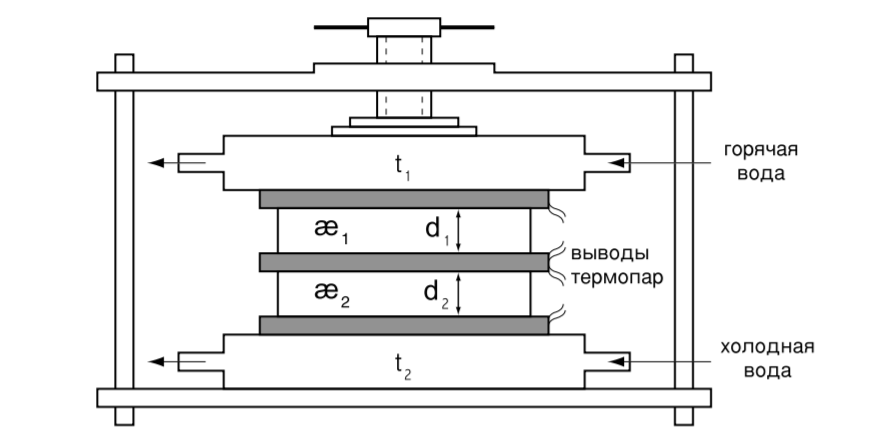
\includegraphics[scale = 0.6]{pic1}}
	\caption{Прибор для измерения коэффициента теплопроводности
сравнительным методом}
	\label{pic:1}
\end{figure}

Две пластинки, изготовленные из материалов с коэффициентами теплопроводности $\varkappa_1$ и $\varkappa_2$, зажимаются между стенками, температуры которых равны $T_1$ и $T_2$ и поддерживаются постоянными во времяопыта. Если толщины пластинок $d_1$ и $d_2$ достаточно малы (по сравнению с наименьшим линейным размером их поверхности), то и потери тепла через боковые поверхности то
же малы. В таком случае площадь теплового потока, протекающего от горячей стенки к холодной, приблизительно остается постоянной (оценка дана ниже). В этом случае

\begin{equation}
	\Delta q =  \varkappa_1 S \frac{\Delta T_1}{\Delta z_1} =  \varkappa_2 S \frac{\Delta T_2}{\Delta z_2},
	\label{eq:2}
\end{equation}

Полагая, что $\Delta z_1 = d_1$ и $\Delta z_2 = d_2$, получим окончательно 

\begin{equation}
	\frac{\varkappa_1}{\varkappa_2} = \frac{d_1}{d_2}\frac{\Delta T_2}{\Delta T_1},
	\label{eq:3}
\end{equation} 

где $\Delta T_1$ и $\Delta T_2$ -- перепады температур на пластинках. Зная теплопроводность материала одной из пластинок, легко определить на опыте
теплопроводность другой пластинки.

\subsection{Оценка потерь тепла}
Формула (\ref{eq:3}) получается в предположении сохранения теплового потока неизменным через обе пластинки, что оправдано при толщине, очень малой по сравнению с радиусом пластинки. Однако хотя и малый, но тепловой поток через боковые поверхности существует всегда. Обнаружить его присутствие можно экспериментально путем измерения распределения температуры. Данные о ее понижении к краю пластинок свидетельствуют о наличии потерь. Использу я такие результаты, покажем, как можно сделать количественную оценку потерь
и найти их относительную величину.

Анализ двумерного распределения температуры основывается на экспериментальных данных о зависимости температуры от радиуса. По ним можно определить плотность радиального потока тепла $q_r$. Это величина есть радиальная компонента вектора $\vec{q}$ и определяется радиальным значением градиента температуры. Полный радиальный поток есть произведение $q_r$ и
площади боковой поверхности $S_r$, вычисленной на том же расстоянии
от оси симметрии, на котором производилось измерение радиальной
производной температуры

\begin{equation}
	q_rS_r=-\varkappa 2 \pi r d \frac{\partial T}{\partial r}.
	\label{eq:4}
\end{equation}

Отношение этих потоков обозначим $\delta$:

\begin{equation}
	\delta = \frac{2d\frac{\partial T}{\partial r}}{r \frac{\partial T}{\partial r}}.
	\label{eq:5}
\end{equation}

Этот параметр характеризует расширение теплового потока и его
относительные потери, он не зависит от коэффициента теплопроводности.

Интересно отметить, что величина $\delta$ не зависит и от радиуса, то есть отношение радиального потока к осевому одинаково и на оси симметрии, и вдали от неё. Расширение осевого теплового потока существует везде, а не только около краев пластинок. Это заключение следует из того, что температура имеет максимум на оси симметрии при любой координате $z$ из-за симметрии пластинок. Поэтому разложение температуры по радиусу от оси начинается с квадратичного члена, следовательно, производная температуры по радиусу в формуле (\ref{eq:5}) пропорциональна радиусу, и этот радиус сокращается с радиусом, который уже есть в знаменателе. Кроме того, при малых потерях через боковые стенки осевой поток тепла изменяется тоже на малую величину, поэтому, и производная $\frac{\partial T}{\partial z}$ изменяется только на малую величину, то есть в первом приближении не зависит от радиуса как и остальные члены формулы (\ref{eq:5}). Отсюда можно сделать вывод, что относительное расширение теплового потока в однородной среде примерно одинаковое на всей пластинке.

\section{Экспериментальная установка}

Прибор для измерения коэффициента теплопроводности (\ref{pic:1}) представляет собой систему из нагревателя, имеющего температуру $T_1$, и холодильника, имеющего температуру $T_2$; эти температуры поддерживаются постоянными. Тепловой поток от нагревателя к холодильнику протекает через зажатые
между ними пластинки из исследуемого и эталонного материала. В качестве эталона удобно было бы использовать эластичный материал, способный создавать надежный тепловой контакт. К сожалению, коэффициент теплопроводности многих эластичных материалов, и в особенности резины, в диапазоне от 0 до 100 ℃ сильно зависит от температуры, поэтому применять резину в качестве эталона крайне неудобно. В нашем приборе эталонным материалом является эбонит, коэффициент теплопроводности которого равен 0,17 Дж/м·с·К. Для получения надежного теплового контакта между поверхностями прокладывается резина.При измерениях коэффициента теплопроводности между нагревателем и холодильником закладываются переложенные тонкими резиновыми прокладками пластинки из исследуемого и эталонного материалов. Вся система сжимается винтовым прессом.
Для стабилизации температур $T_1$ и $T_2$ через холодильник постоянно пропускается проточная вода из водопровода (вентиль на столе за прибором), а через нагреватель циркулирует горячая вода, поставляемая термостатом. Измерение температур производится при помощи четырех термопар, рабочие спаи которых помещают в середине пластинок. Спаи двух термопар прижимают резиновыми прокладками к обеим сторонам эталонной пластинки, спаи двух других -- к пластинке из исследуемого материала. Вторые спаи термопар помещены в пробирку с маслом, омываемую водопроводной водой. При этих условиях температура холодных спаев термопар за время эксперимент а практически не меняется

Переключатель позволяет поочередно подключать термопары к зеркальному гальванометру. Показания гальванометра пропорциональны разности температур рабочего и холодного спаев термопар. Измерив температуры обеих поверхностей пластинки, можно вычислить перепад температуры на пластинке. Прежде чем приступить к измерениям, необ ходимо включить термостат (перевести движок переключателя в верхнее положение) и его нагревательно-смешивающий узел (кнопкой «Pump»).

Для увеличения скорости нагрева регулятор мощности нагревателя (Heatinq
Power adjustment) следует поставить в крайнее правое положение. (При приближении температуры воды к 70 ℃ регулятор переводится в крайнее левое положение).

Вращая головку контактного термометра, установите температуру выше 70 ℃. В момент, когда контрольный термометр покажет 70 ℃, нужно, медленно вращая головку контактного термометра, выключить нагреватель. При выключении гаснет красная контрольная лампочка.

Если к вашему приходу термостат уже включен и установлен на нужную температуру, то следует сразу перейти к выполнению задания.

\section{Ход работы}

\subsection{Время установления равновесного теплового потока}

Данные установки: $t_{\text{гор}} = 70 \pm 0.1$ ℃, $t_{\text{хол}} = 5 \pm 0.1$ ℃.

Экспериментально оценим время установления равновесного теплового потока в система. Для этого снимим зависимость температуры какой-либо точки от вермени и по графику, построенному по результатам наших измерений, оценим величину времени установления. Так же все последующие измерения будем проводить после установления равновесных условий в установке.

Оценивать будем по следующей формуле:

\begin{equation}
	x^2 = t \chi
	\label{prob:1}
\end{equation}

Для этого по справочкнику определим среднее значение коэффициента температуропроводности для набора пластинок или просто используем какое-нибудь одно значение. Далее сравним рассчитанное время с измеренным.

По полученным данным получаем, что время установления: $\tau_{\text{уст}} \approx (238 \pm 1.5)  \text{с}$ .

Из табличных значений, пользуясь формулой (\ref{prob:1}) расчитаем время установления :
\[ \chi = \frac{\varkappa}{\rho c_V} = \frac{0.162}{1680 \cdot 1430} . \approx 6,74 \cdot 10^{-8} [\text{м}^2 / \text{с}] \Rightarrow \tau_{\text{уст}} \approx 237\ [c]\]

Тогда можно оценить коэф. температуропроводности эбонита: $\chi = \frac{x^2}{\tau_{\text{уст}}} = 6.72 \cdot 10^{-8} [\text{м}^2 / \text{с}]$. Видно, что времена установления практически идентичны.
\subsection{Калибровка термопары}

Прокалибруем применяемые в работе термопары. Для этого рабочие спаи всех термопар расположим в одной точке прибора (например, прижмем к середине одной из сторон эбонитовой пластинки). Необходимо следить, чтобы провода от каждой термопары шли параллельно и не касались друг друга. Показания гальванометра при подключении его к различным термопарам пропорциональны чувствительности термопар, которые могут несколько отличаться из-за различия в сопротивлениях спаев.

Если показания гальванометра $a_1, a_2, a_3, a_4$ будут заметно отличаться друг от друга, то отношение, входящее в формулу (\ref{eq:3}), будем вычислять по следующей формуле:

\begin{equation}
	\frac{\Delta T_2}{\Delta T_1} = \frac{\varphi_4/a_4 - \varphi_3/a_3}{\varphi_2/a_2 - \varphi_1/a_1},
	\label{eq:6}
\end{equation}

где $\varphi_1, \varphi_2, \varphi_3, \varphi_4$ -- показания гальванометра, полученные во время опыта по измерению коэффициента теплопроводности. В этой формуле индексы при $a$ и $\varphi$ характеризуют номер термопары. Величины $a_i$ и $\varphi_i$ получим при подключении гальванометра к одной и той же термопаре.

В данном эксперименте было получено, что чувствительность термопар практически идентична. И скорее всего различие в значении скорее всего обусловлено тем, что какие-то термопары были ближе к центру диска, а какие-то более даленные. Полученные значения для коэффициентов $a_1 = 1.17, a_2 = 1.17, a_3 = 1.16, a_4 = 1.17$. Поэтому далее отношение $\frac{\Delta T_2}{\Delta T_1}$ будем считать без учета разных чувствительностей термопар. 

\subsection{Проверка предположения}
Проверим на опыте, в какой мере выполняется предположение о независимости коэффициента теплопроводности эталонного материала от температуры. Для этого в прибор зажмем пакет из двух одинаковых слоев пластинок эбонита, переложенных резиновыми прокладками. С помощью термопар измерим разности температур на эбонитовых слоях. Эти слои находятся в различных температурных условиях. Если коэффициент теплопроводности не зависит от температуры, разности температур на слоях, как это следует из (\ref{eq:3}) должны быть пропорциональны их толщинам.  Толщину пластинок измерим штангенциркулем. 

Полученные толщины пластинок (были использованы два диска из эбонита): $d_1 = 4 \textbf{мм}$, $d_2 = 4 \textbf{мм}$. Далее установим термопары в соответствующие места и дождемся термодинамического равновесия. После установления снимаем значения на термопарах: $\varphi_2 = 1.29, \varphi_1 = 0.19 \Rightarrow \Delta T_1 = \varphi_2 - \varphi_1 = 1.1$. Аналогично посчитаем значения для $\Delta T_2 = \varphi_4 - \varphi_3 = 2.1 - 0.99 = 1.11$. Тогда по формуле (\ref{eq:3}) получим, что $\frac{\varkappa_1}{\varkappa_2} = \frac{0.4}{0.4}\frac{\Delta T_2}{\Delta T_1} \approx 1.$ Отсюда можно сделать вывод об справедливости предположения о независимости коэффициента теплопроводности эталонного материала от температуры.  
\subsection{Основной опыт}
После того, как мы провели предварительные эксперименты, можем приступить к основному опыту. Измерем коэффициенты тепловодности образцов (плексиглас, текстолит, гетакс). По показаниям гальванометра и по чувствительности термопар определим для каждого образца отношение разностей температур на образце и на эбоните согласно формуле (\ref{eq:6}) (ранее было определено, что можно рассчитывать по обычной формуле, так как чувствительности у термопар идентичны), а затем используем формулу (\ref{eq:3}).
Для начала приведем таблицу толщин дисков:
\begin{center}
\begin{tabular}{|c|c|c|c|c|c|}
\hline 
 & Плексиглас & Гетинакс & Текстолит & Стеклотекстолит & Эбонит \\ 
\hline 
d, мм & 4.5 & 4.5 & 4.1 & 3.0 & 4.0\\ 
\hline 
\end{tabular}
\end{center} 

Теперь таблицу значений $\varphi_i$ для каждого из экспериментов (сначала исследуемое тело снизу, потом сверху, а $t_1, ... , t_4$ -- всегда установлены одинакого относительно установки, а именно $t_1$ между нижней резиной и нижним диском, $t_2$ выше нижнего диска и между резиной, $t_3$ под верхним диском и над резиной, $t_4$ сверху верхнего диска).

\begin{center}
\begin{tabular}{|c|c|c|c|c|c|c|c|}
\hline 
\multicolumn{2}{|c|}{Плексиглас} & \multicolumn{2}{c|}{Гетинакс} & \multicolumn{2}{c|}{Текстолит} & \multicolumn{2}{c|}{Стеклотекстолит} \\ 
\hline 
$\varphi_1$ & 0.20 & $\varphi_1$ & 0.29 & $\varphi_1$ & 0.21 & $\varphi_1$ & 0.21 \\ 
\hline 
$\varphi_2$ & 1.15 & $\varphi_2$ & 1.04 & $\varphi_2$ & 1.00 & $\varphi_2$ & 0.77 \\ 
\hline 
$\varphi_3$ & 1.26 & $\varphi_3$ & 1.06 & $\varphi_3$ & 1.00 & $\varphi_3$ & 0.50 \\ 
\hline 
$\varphi_4$ & 2.21 & $\varphi_4$ & 2.02 & $\varphi_4$ & 2.08 & $\varphi_4$ & 2.08 \\ 
\hline 
$\frac{\Delta T_1}{\Delta T_2}$ & 1.00 & $\frac{\Delta T_1}{\Delta T_2}$ & 1.28 & $\frac{\Delta T_1}{\Delta T_2}$ & 1.367 & $\frac{\Delta T_1}{\Delta T_2}$ & 2.82 \\
\hline
\end{tabular}
\end{center} 

\begin{center}
\begin{tabular}{|c|c|c|c|c|c|c|c|}
\hline 
\multicolumn{2}{|c|}{Плексиглас} & \multicolumn{2}{c|}{Гетинакс} & \multicolumn{2}{c|}{Текстолит} & \multicolumn{2}{c|}{Стеклотекстолит} \\ 
\hline 
$\varphi_1$ & 2.07 & $\varphi_1$ & 1.88 & $\varphi_1$ & 2.00 & $\varphi_1$ & 1.96 \\ 
\hline 
$\varphi_2$ & 0.96 & $\varphi_2$ & 1.37 & $\varphi_2$ & 1.25 & $\varphi_2$ & 1.50 \\ 
\hline 
$\varphi_3$ & 0.94 & $\varphi_3$ & 1.38 & $\varphi_3$ & 1.21 & $\varphi_3$ & 1.58 \\ 
\hline 
$\varphi_4$ & 0.13 & $\varphi_4$ & 0.19 & $\varphi_4$ & 0.16 & $\varphi_4$ & 0.24 \\ 
\hline 
$\frac{\Delta T_1}{\Delta T_2}$ & 0.73 & $\frac{\Delta T_1}{\Delta T_2}$ & 2.38 & $\frac{\Delta T_1}{\Delta T_2}$ & 1.40 & $\frac{\Delta T_2}{\Delta T_1}$ & 2.91 \\
\hline
\end{tabular}
\end{center}

Погрешность полученных значений для $\frac{\Delta T_1}{\Delta T_2}$ обусловленная погрешностью измерений гальванометра. 

Из данных таблиц, используя формулу (\ref{eq:3}) и значение коэффициента теплопроводности эталонного тела ($\chi = 0.162$) найдем значения коэффициентов для исследуюмых тел. Так же можем сравнить их со значениями, данных нам в таблицах и судить о зависимости этих коэффициентов от температуры, так как проводилось 2 серии опытов, как описалывалось уже выше.

\begin{center}
\begin{tabular}{|c|c|c|c|}
\hline 
Исследуемый предмет & $t, ^\circ C$ & Эксп. значение & Теор. значение \\ 
\hline 
Плексиглас & 20 & 0.182 & 0.184 \\ 
\hline 
Гетинакс   & 20 & 0.233 & 0.24 \\ 
\hline 
Текстолит  & 20 & 0.227 & 0.233-0.337 \\ 
\hline 
Стеклотекстолит & 20 & 0.342 & 0.372 \\ 
\hline 
\end{tabular} 
\end{center}

Погрешность полученных значений обусловленна погрешностью измерений толщины пластинок, погрешностью измерений показаний с гальванометра, так же погрешность расчетов и округлений.

По результатам сравнения $\frac{\Delta T_2}{\Delta T_1}$ при разном расположении исследуемого тела и эталонного можно сделать вывод, что от температуры коэф. теплопроводности зависит у плексиглаза и гетинакса, а у текстолита и стеклотекстолита практически не зависит.

\subsection{Оценка потерь через боковые поверхности}
Потери через боковые поверхности оценим с помощью следующего опыта. Разместим рабочие спаи термопар на разных расстояниях от центра пластины, например, на расстояниях 0, 1, 2, 3 см или одну в центре, другую с краю и остальные между ними. Запишим эти расстояния, они потребуются при обработке результатов. Чтобы избежать ошибок, связанных с теплоотводом через провода термопар в этом точном эксперименте, длины всех прижатых частей проводов будем стараться делать одинаковыми. С помощью гальванометра измерим температуры. Уменьшение температуры при удалении от центра обусловлено тепловым потоком через боковые поверхности. По графику найдем производную температуры по радиусу (в единицых показаний гальванометра, поделенных на соответствующую чувствительность).

Производную будем определять ближе к краю пластинки, там измерения точнее. Можно также воспользоваться интерполяцией по графику и даже экстраполяцией к краю пластинки. 

Осевую производную температуры найдем по рабочим измерениям в другом опыте с той же пластинкой, но при расположении термопар не вдоль радиуса, а вдоль оси симметрии.

Используя полученные из опыта величины для расчеты относительных потерь тепла по формуле (\ref{eq:5}).

Так как всего термопар 4, а точек снять хочется больше, то будем снимать их в 2 захода: сначала снимем значения на 4 точках с расстояниями 0, 1, 2, 3 см соответственно от центра, а затем аналогично еще 2 точки (4, 5 см от центра), потому что радиус диска 5.1 см, то больше точек снять мы не можем. Полученная таблица результатов (сразу стоит заметить, что при проведении опыта сильным фактором являлось расположение концов термопар, в связи с этим велика вероятность, что полученные данные имеют большую погрешность):

\begin{center}
\begin{tabular}{|c|c|c|c|c|c|c|}
\hline
$i$ & $1$ & $2$ & $3$ & $4$ & $5$ & $6$ \\ 
\hline 
$\varphi_i$ & 1.10 & 1.09 & 1.08 & 1.05 & 1.00 & 0.92\\ 
\hline 
$r_i$ & 0 & 1 & 2 & 3 & 4 & 5\\ 
\hline 
\end{tabular} 
\end{center}

Построим график полученной зависимости ($\varphi (r)$):
\newpage
\begin{figure}
	\center{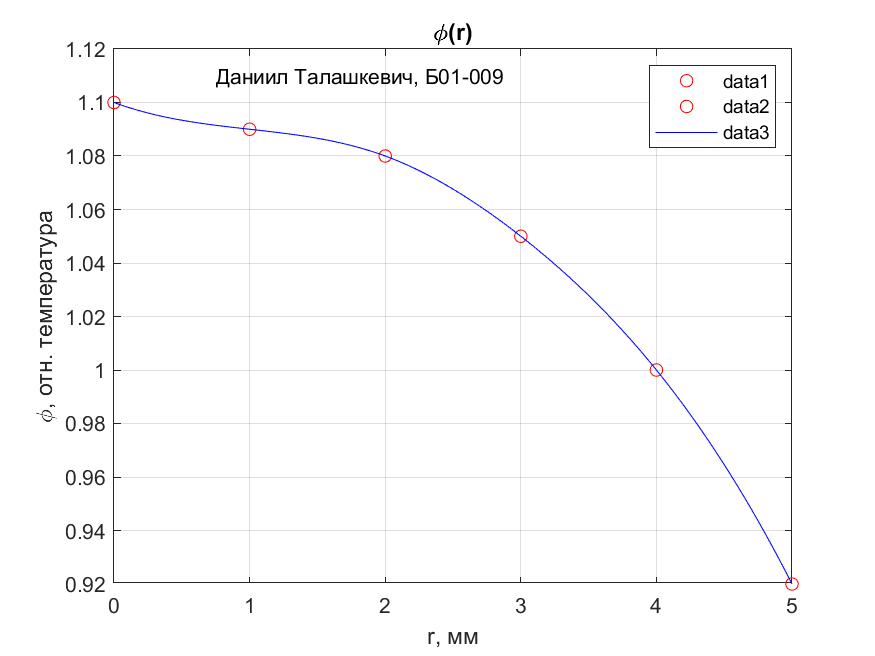
\includegraphics[scale = 0.6]{graph1.png}}
	%\caption{Сферическая система координат наглядно}
	\label{gr:1}
\end{figure}

Отсюда получено значение $\frac{\partial \varphi}{\partial r} = 0.06 \ [\text{ отн. темп} / \text{мм }].$

Осевую производную можно определить по данным из пункта 3, так как там мы как раз и измеряли зависимость температуры от осевого расстояния. По этим данным выше приведен график зависимости:

\begin{figure}
	\center{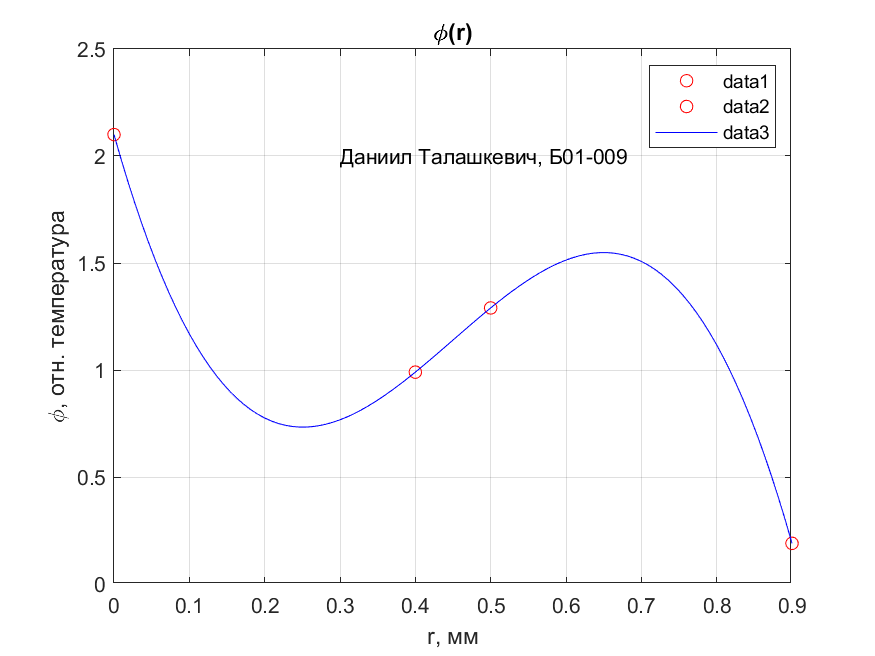
\includegraphics[scale = 0.6]{graph2.png}}
	%\caption{Сферическая система координат наглядно}
	\label{gr:2}
\end{figure}

И соответственное значение в близи к центру $\frac{\partial \varphi }{\partial z} = 0.334 \ [\text{ отн. темп} / \text{мм }].$

Тогда без труда определим относительные потери тепла по следующей формуле:

\[ \delta = \frac{2d \frac{\partial T}{\partial r}}{r \frac{\partial T}{\partial z}}  = \frac{2 \cdot 4 \cdot 0.06}{51 \cdot 0.334} = 2.8 \cdot 10^{-2} .\]


\section{Вывод}
Построенная нами модель полностью оправдала себя, ведь мы смогли практически точно измерить коэффициента температуропроводности исследуюмых тел путем сравнения с эталонным материалом и определить у каких материалов коэф. теплопроводности зависит от температур, а у каких нет. Так же мы вычислили относительные тепловые потери через боковые поверхности.

В общем случае, количество тепла, выделяемое в объёме $d V$, определяется соотношением
$$
d Q^{T}=-\tau(\nabla T \cdot \mathbf{j}) d t d V
$$

\begin{figure}[h]
%	\center{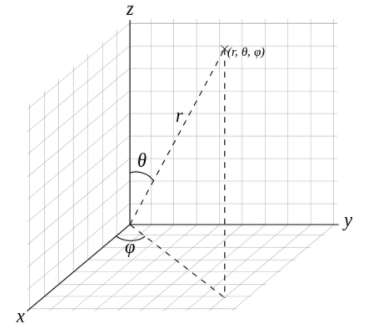
\includegraphics[scale = 0.75]{pictures/Angles}}
%	\caption{Сферическая система координат наглядно}
%	\label{Angles}
\end{figure}


					\end{document}
